\chapter{Prototipo funcional V2}\label{proto2}

Luego de un primer prototipo, se analiza el funcionamiento general para planificar cambios y mejoras necesarias. Entre las que destacan un control sobre el envío de datos desde los sensores y una optimización de código en Arduino (relevante por la baja frecuencia de operación que posee frente a las exigencias del proyecto).

Los detalles se presentan a continuación, aunque adelantando que los cambios principales de esta nueva versión fueron realizados a la programación del microcontrolador y su sincronización con la aplicación.

\section{Control de sensores por Android}

Un aspecto fundamental para el proyecto es la posibilidad de controlar el inicio y el fin de las mediciones desde la aplicación, permitiendo en una iteración posterior su control desde la web.

Para este efecto, se desarrolla un protocolo de comunicación con el cual se espera sincronizar las acciones entre los dos principales entes (microcontrolador con módulo Bluetooth y aplicación Android).

Se comienza estableciendo un conjunto de instrucciones homogéneas con las cuales los dispositivos puedan ejecutar órdenes:

\textbf{00}: Detener medición

\textbf{10}: Iniciar solo medición de ECG

\textbf{01}: Iniciar solo medición de T

\textbf{11}: Iniciar ambas mediciones \newpage

Como se puede observar, se utiliza un sistema binario en el cual con 2 bit se logran controlar 4 estados fundamentales. Se escoge esta arquitectura dada su fácil escalabilidad y sencilla comprensión al asignar 0 o 1 a cierta posición asociada (y preacordada) a algún sensor.

Esto en conjunto con un Handler (ejecución de una tarea en otro hilo) en Android, permite el control temporal de estas instrucciones. Logrando así que al momento que la aplicación recibe una petición de medicón, ésta sea comandada por el Handler que a su vez tiene un Timer asociado, con el cual se podrá controlar la ejecución de la medición por una cantidad de tiempo preestablecida.

\begin{figure}[H]
	\centering
	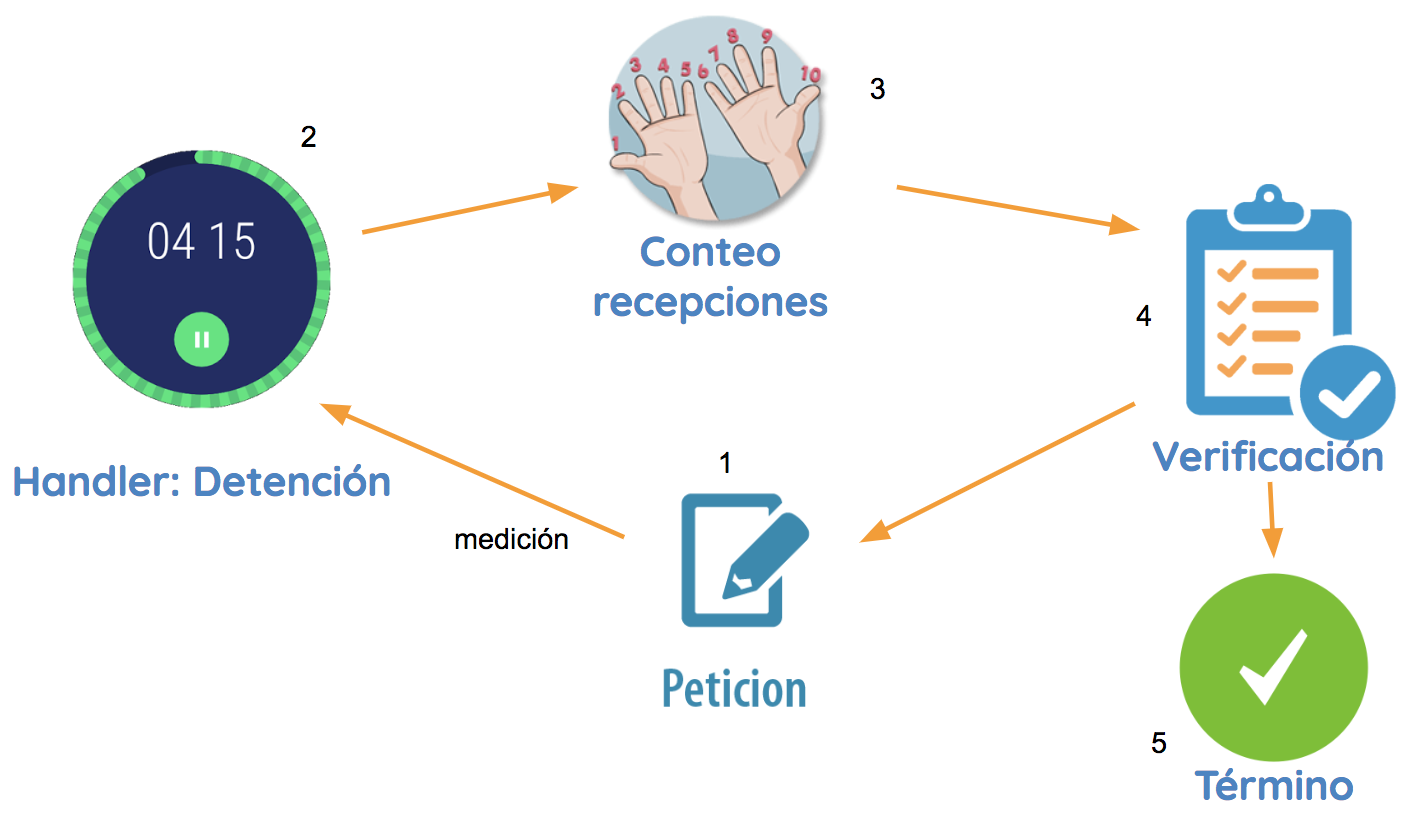
\includegraphics[scale=0.5]{figuras/proto2/handler.png}
	\caption{Control de peticiones por Handler y repetición}
	\label{handler}
\end{figure}

En la figura \ref{handler} se pueden observar los distintos estados asociados a una medición: Petición, medición, detención, conteo, verificación y término.

Al acabar con la medición, el microcontrolador comunica la cantidad de paquetes enviados asociados a cada sensor, cantidad que es verificada con los recibidos en la aplicación y dependiendo de esto último se repite la petición de forma automática o se da por terminada la medición. \newpage

Las secuencias de control corresponden a una cadena de caracteres compuesto por AA y FF al inicio y término respectivamente de una medición, seguidos por 4 caracteres contenedores de 2 byte hexadecimales con el número de paquetes enviados (0 a 65536 paquetes).

Esto último supone una restricción en la cantidad máxima de paquetes enviados por medición:

\textbf{ECG}: Con una tasa de 150 [Hz] | Máximo 6.8 minutos por medición.

\textbf{T}: Con una tasa de 1 [Hz] | Máximo 18.2 horas por medición.

\section{Renovación de servidor Arduino}

Considerando la opción de microcontrolador escogido (Arduino UNO), se tiene una limitante importante en cuanto a la potencia de procesamiento presente, la cual se limita a la frecuencia de operación con la que cuenta el chip ATmega328 que es de 16 [MHz]. 

Por esta razón se hace indispensable una programación prolija y con miras en la optimización en la ejecución de instrucciones. En este sentido, se realizan diversos cambios al código fuente del microcontrolador (se pueden ver con detalle en los Anexos):

Control del ciclo principal de operación bajo milisegundos a microsegundos.

Uso de punteros en vez de copia de memoria para el manejo de arreglos de char.

Uso de condiciones según precedencia y uso de else if según casos más frecuentes.

Control de estados por variables, minimizando verificaciones innecesarias.

\newpage

\section{Análisis de resolución y frecuencia para ECG}

Pasando directamente al manejo del ECG por parte del controlador, se realizan pruebas para establecer frecuencias necesarias y verificar nivel de resolución mínimas, entre las que se destacan los siguientes resultados.

\begin{figure}[H]
	\centering
	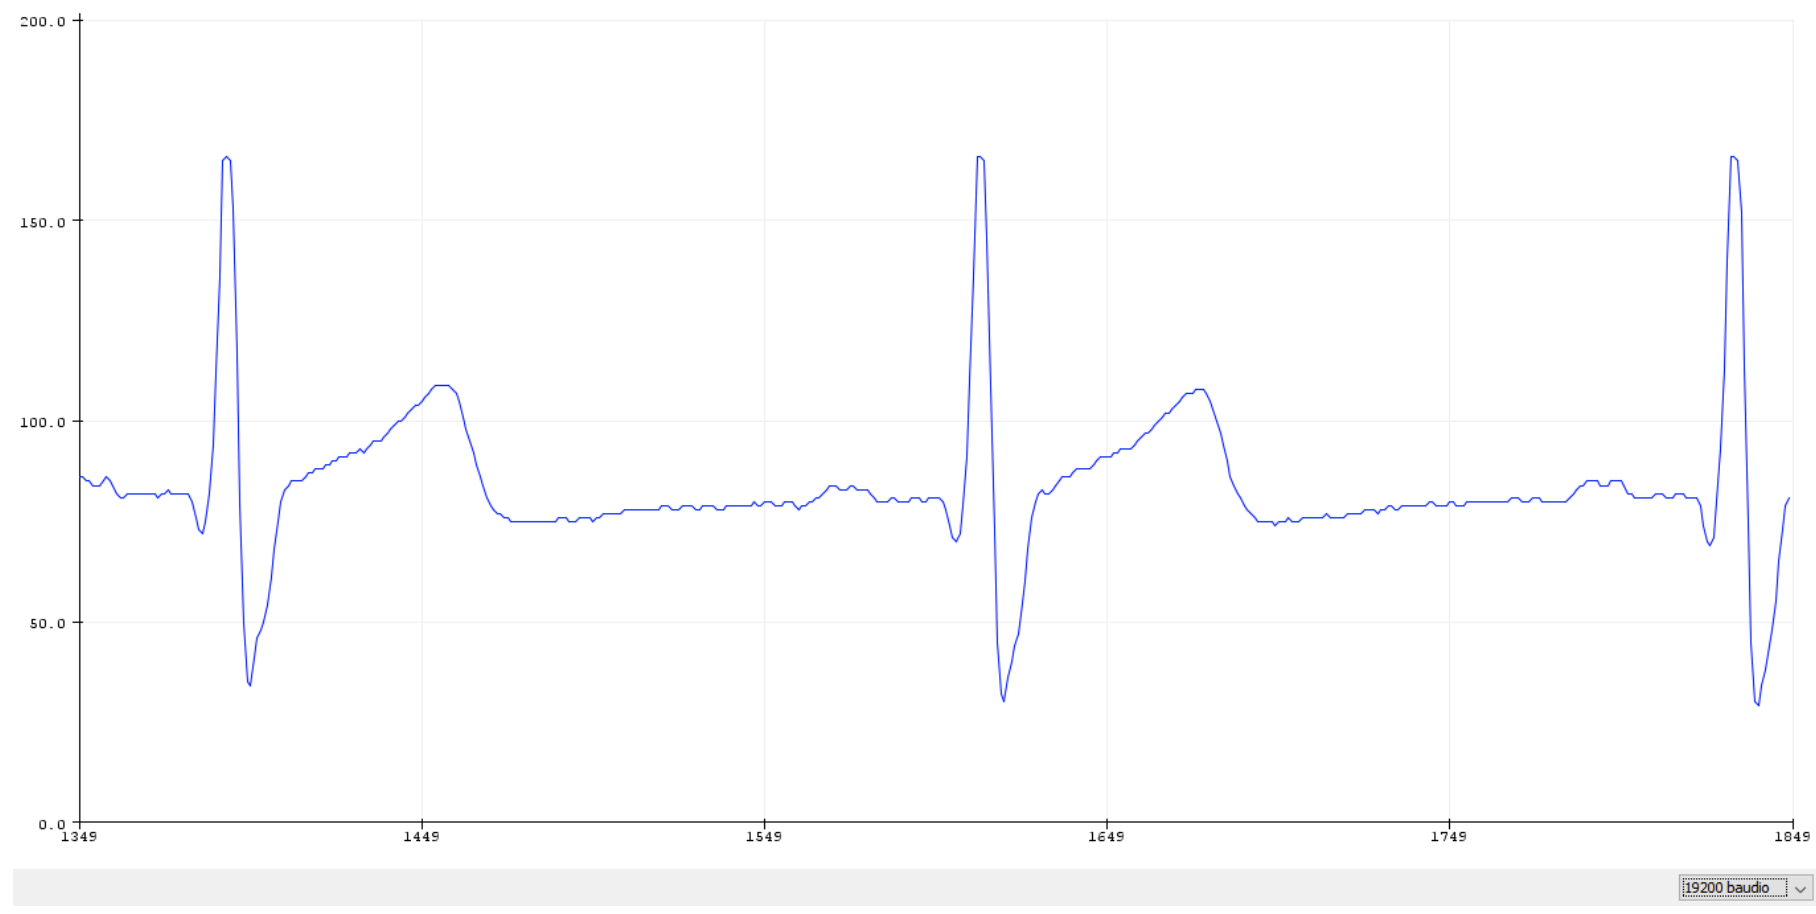
\includegraphics[scale=0.4]{figuras/proto2/8bit.png}
	\caption{ECG a 300 [Hz] y 8 bit de resolución}
	\label{8bit}
\end{figure}

\begin{figure}[H]
	\centering
	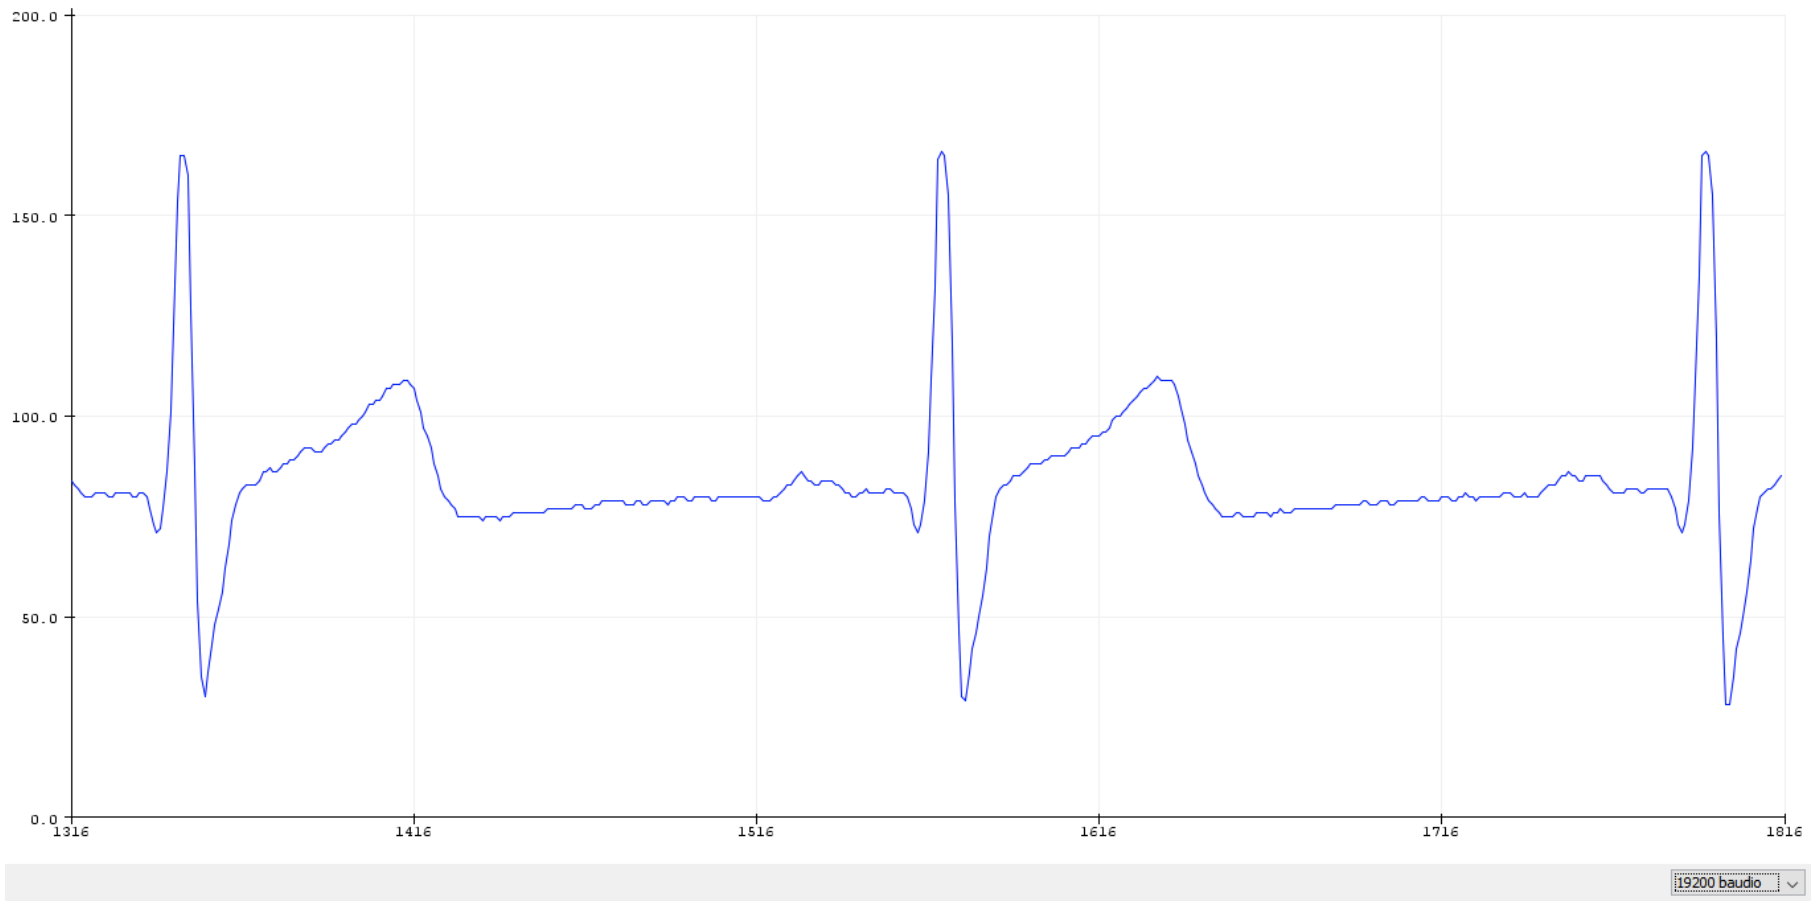
\includegraphics[scale=0.4]{figuras/proto2/10bit.png}
	\caption{ECG a 300 [Hz] y 10 bit de resolución}
	\label{10bit}
\end{figure}

\newpage

Como se puede obervar en las figuras anteriores, la resolución obtenida utilizando 8 bit o 10 bit no representa un cambio significativo a nivel visual, mientras que a nivel de procesamiento y almacenamiento sí posee gran injerencia (valor máximo: 256 y 1024 respectivamente). 

Esto es especialmente importante cuando se tiene en cuenta que la comunicación hexadecimal funciona de forma óptima con información condensada en múltiplos de 8 bit, puesto que la representación de 1 byte (8 bit) es posible por medio de solo 2 caracteres hexadecimales que son exactamente el byte de información.

Así, se decide emplear esta resolución para la captura y comunicación de los datos de ECG, sin miedo a perder información o tener sobrecarga de caracteres, en una comunicación con paquetes contenedores más grandes que la información mínima.

Se hicieron pruebas de frecuencia para el ECG, probando valores entre 50 [Hz] y 1.000 [Hz]. Como resultado de esto se estableció un mínimo de 50 [Hz] de operación, una base esperable de 150 [Hz] y un máximo de 300 [Hz], los anteriores valores por condensación visual de los datos (se observa una compresión horizontal de las gráficas a menores frecuencias y lo contario para frecuencias mayores).

\begin{figure}[H]
	\centering
	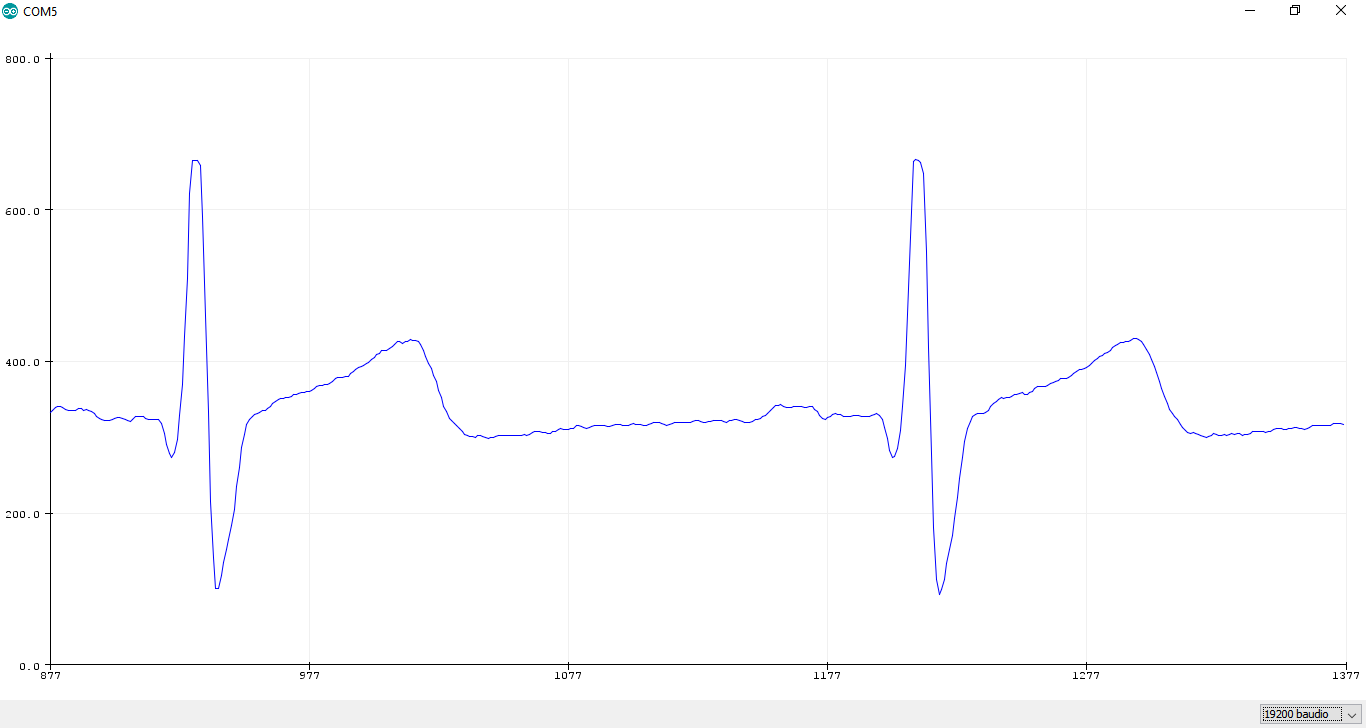
\includegraphics[scale=0.4]{figuras/proto2/1000hz.png}
	\caption{ECG a 1.000 [Hz] y 10 bit de resolución}
	\label{1000hz}
\end{figure}

\section{Base de datos local (comparativa Realm, SQLite) }

De nada sirve obtener y comunicar datos si estos no son almacenados y estudiados posteriormente, es por ello que se contempló desde el inicio del proyecto el uso de una base de datos local para la aplicación (útil especialmente para mediciones sin cobertura) y una base de datos propia del servidor web.

En Android existen principalmente dos grandes alternativas respecto a bases de datos: SQLite y Realm (ambas relacionales y con esquema llave-valor). La primera de ellas, SQLite es un motor de base datos ampliamente utilizada y disponible desde los inicios del SO Android, sus grandes ventajas son la gran penetración que ya posee en los desarrolladores y los distintos sabores entenidos en las librerías que lo implementan.

La segunda alternativa es relativamente nueva pero con un potencial enorme, dada su facilidad de uso, gran rendimiento, visualización de datos con aplicaciones externas, disponibilidad en múltiples SO y su excelente documentación.

A continuación se presentan gráficas provistas por el equipo de Realm en comparativas de rendimiento \cite{realm_android} frente a distintas librerías en Android (en todas más alto es mejor).

 \begin{figure}[H]
 	\centering
 	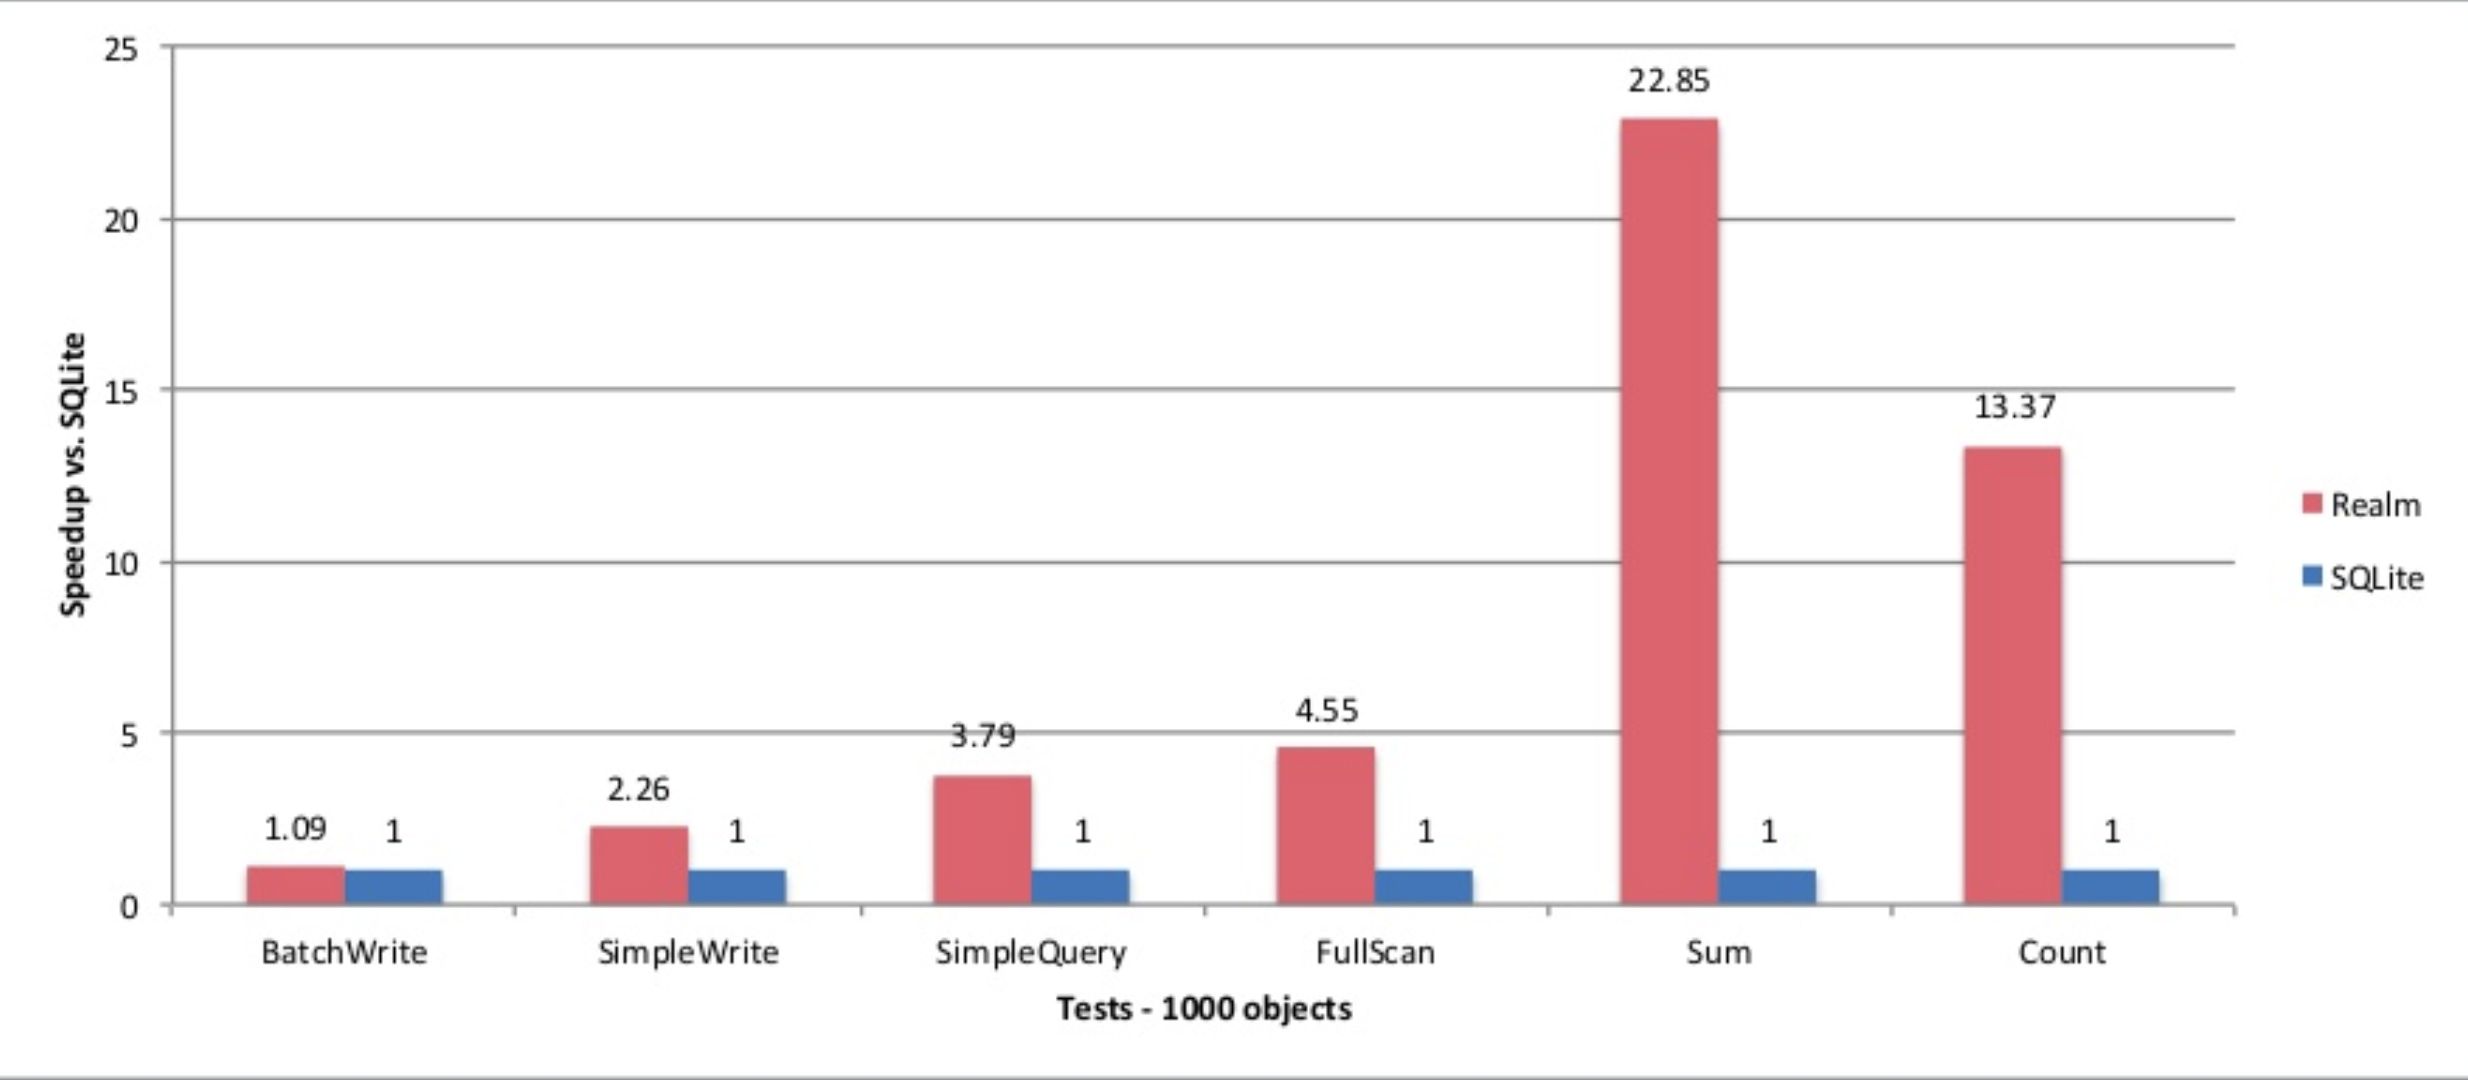
\includegraphics[scale=0.3]{figuras/proto2/benchmark.png}
 	\caption{Benchmark frente a SQLite con el uso de distintas librerías}
 	\label{benchmark_realm}
 \end{figure}

\begin{figure}[H]
	\centering
	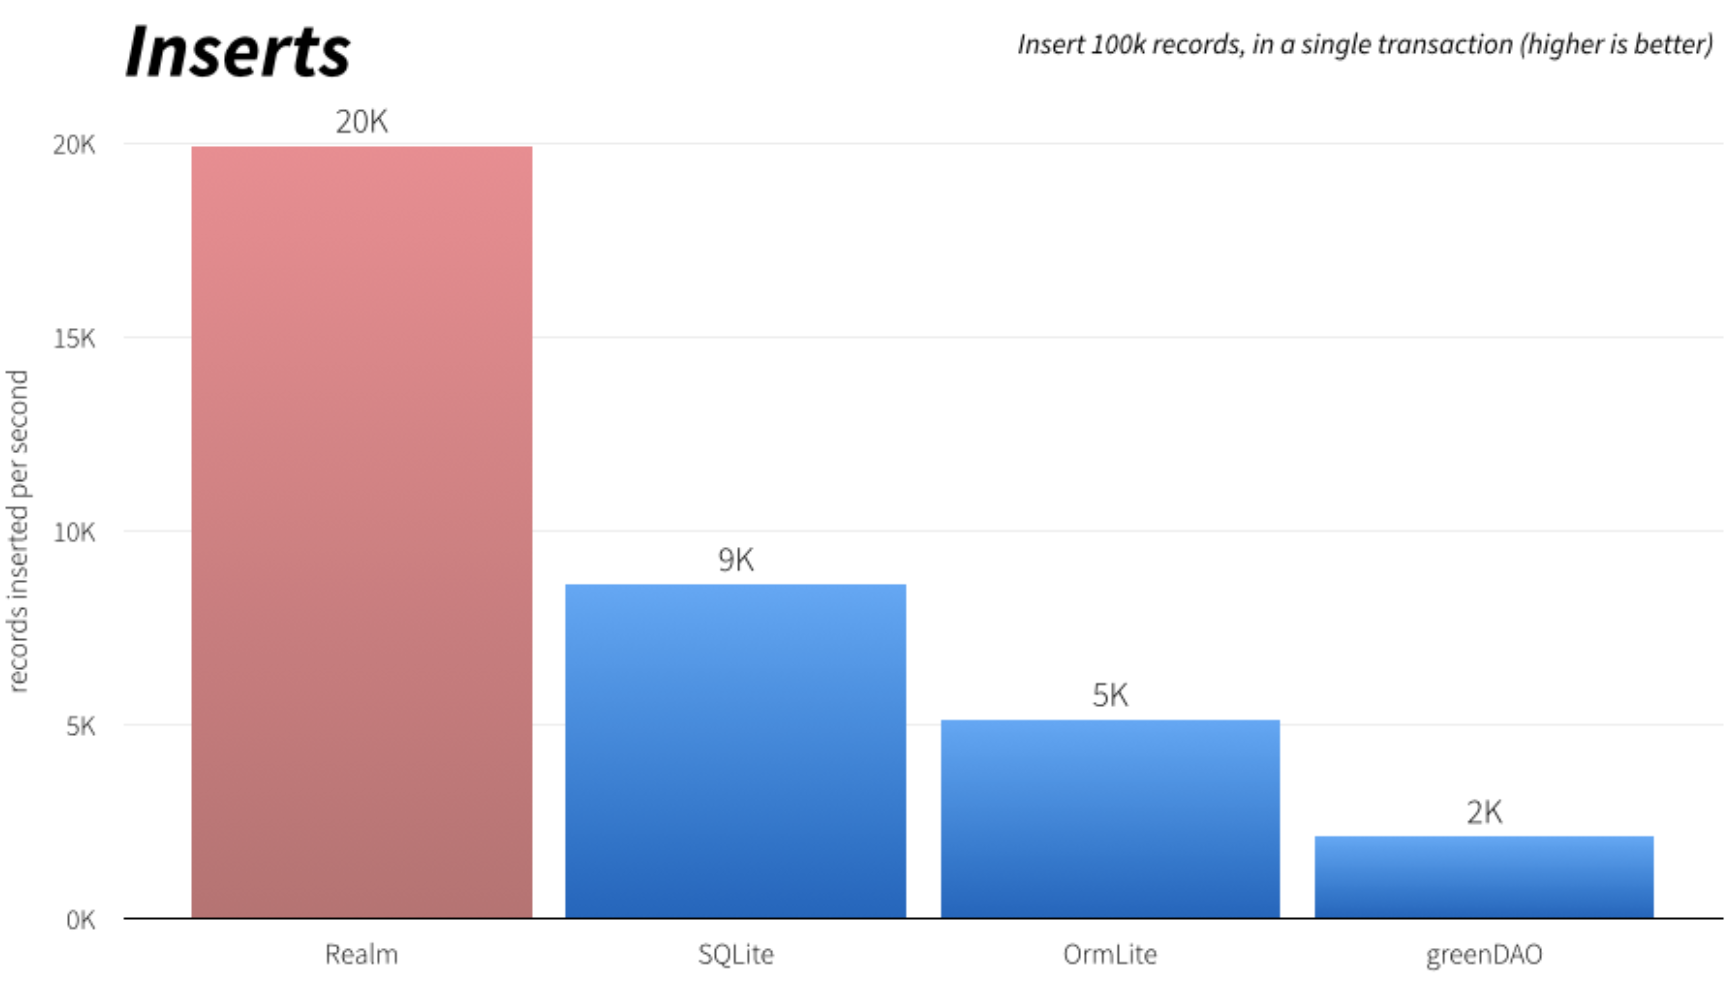
\includegraphics[scale=0.4]{figuras/proto2/insert.png}
	\caption{Comparativa en escrituras a la base de datos}
	\label{insert}
\end{figure}

\begin{figure}[H]
	\centering
	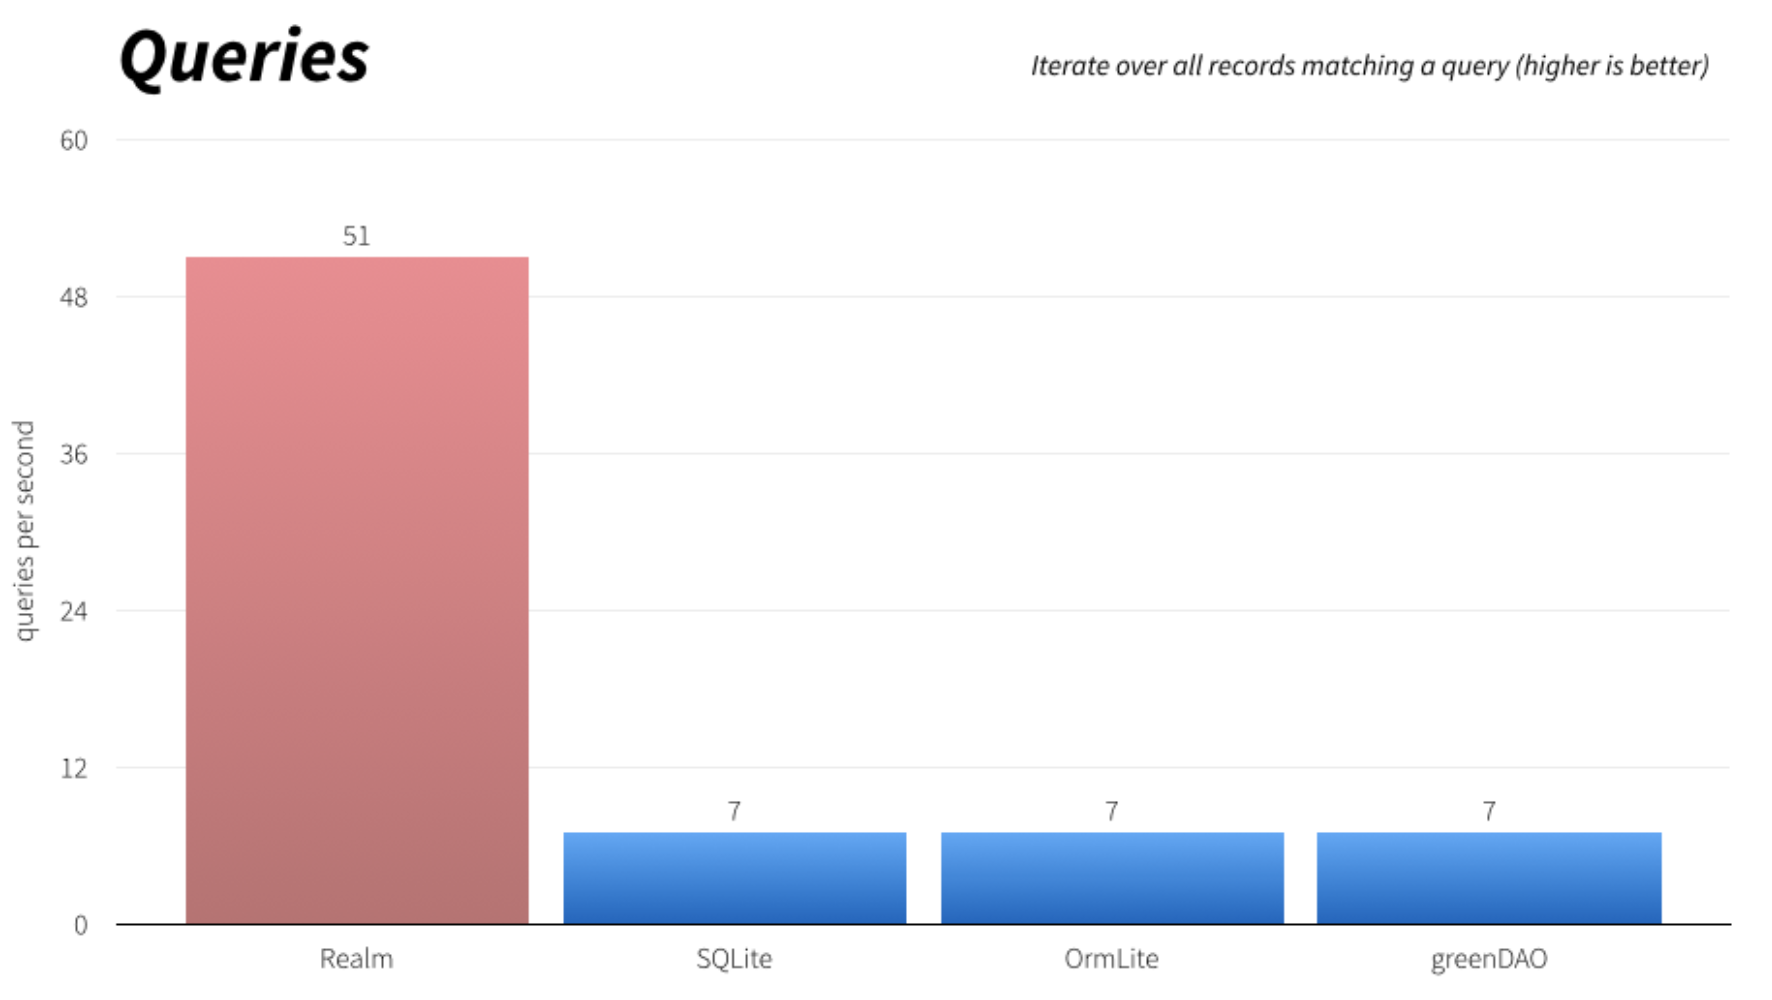
\includegraphics[scale=0.4]{figuras/proto2/queries.png}
	\caption{Comparativa en lecturas a la base de datos}
	\label{queries}
\end{figure}

Es por las figuras anteriores y su resultado apabullante que se hace uso de Realm y no de otra base de datos local. Cabe mencionar que al ser más reciente, posee características interesantes como un manejo sencillo de hilos, instancias, creación de arreglo de objetos, entre otros.

\newpage

\section{Modelo tentativo para Realm}

Si bien no se alcanza a implementar la base de datos ya escogida, se articula un modelo tentativo de las tablas que contendrán la información de las mediciones. Estableciendo de esta manera los datos y la relación presente entre ellos, se presenta la llave primaria en negrita para cada tabla.

\begin{table}[H]
	\centering
	\begin{tabular}{| c | c |}
		\hline
		\multicolumn{1}{|c|}{\textit{Dato}}&
		\multicolumn{1}{c|}{\textit{Tipo}}\\ \hline
		\textbf{Rut}  & String   \\ \hline
		Nombre  & String  \\ \hline
		Sexo & String  \\ \hline
		MAC & String  \\ \hline
		Hospital & String  \\ \hline
		Código Sistema & int  \\ \hline
		Edad & int  \\ \hline
		Teléfono & int  \\ \hline
		Teléfono emergencia & int  \\ \hline
		Teléfono emergencia 2 & int  \\ \hline
		Nº Ficha & int  \\ \hline
	\end{tabular}
	\caption{Tabla Paciente: Datos personales del paciente}
	\label{tabla_paciente}
\end{table}

\begin{table}[H]
	\centering
	\begin{tabular}{| c | c |}
		\hline
		\multicolumn{1}{|c|}{\textit{Dato}}&
		\multicolumn{1}{c|}{\textit{Tipo}}\\ \hline
		\textbf{Rut}  & String   \\ \hline
		\textbf{Fecha\_hora\_min\_seg}  & String  \\ \hline
		Duración & int  \\ \hline
		Sensores & int  \\ \hline
	\end{tabular}
	\caption{Tabla Mediciones: Al iniciar una medición almacena los datos relacionada a esta por posible retransmisión necesaria hacia el servidro web}
	\label{tabla_mediciones}
\end{table}

\begin{table}[H]
	\centering
	\begin{tabular}{| c | c |}
		\hline
		\multicolumn{1}{|c|}{\textit{Dato}}&
		\multicolumn{1}{c|}{\textit{Tipo}}\\ \hline
		\textbf{Rut}  & String   \\ \hline
		\textbf{Fecha\_hora\_min\_seg}  & String  \\ \hline
		Duración & int  \\ \hline
		Enviado & boolean  \\ \hline
	\end{tabular}
	\caption{Tabla ECG: Al iniciar una medición de ECG}
	\label{tabla_ECG}
\end{table}

\begin{table}[H]
	\centering
	\begin{tabular}{| c | c |}
		\hline
		\multicolumn{1}{|c|}{\textit{Dato}}&
		\multicolumn{1}{c|}{\textit{Tipo}}\\ \hline
		\textbf{Fecha\_hora\_min\_seg}  & String  \\ \hline
		\textbf{Contador}  & int  \\ \hline
		Valor & int  \\ \hline
	\end{tabular}
	\caption{Tabla Datos ECG: Se escribe con cada dato, pero asociado a una medición(Fecha\_hora\_min\_seg)}
	\label{tabla_datos_ECG}
\end{table}

\begin{table}[H]
	\centering
	\begin{tabular}{| c | c |}
		\hline
		\multicolumn{1}{|c|}{\textit{Dato}}&
		\multicolumn{1}{c|}{\textit{Tipo}}\\ \hline
		\textbf{Rut}  & String   \\ \hline
		\textbf{Fecha\_hora\_min\_seg}  & String  \\ \hline
		Duración & int  \\ \hline
		Enviado & boolean  \\ \hline
	\end{tabular}
	\caption{Tabla T: Al iniciar una medición de T}
	\label{tabla_T}
\end{table}

\begin{table}[H]
	\centering
	\begin{tabular}{| c | c |}
		\hline
		\multicolumn{1}{|c|}{\textit{Dato}}&
		\multicolumn{1}{c|}{\textit{Tipo}}\\ \hline
		\textbf{Fecha\_hora\_min\_seg}  & String  \\ \hline
		\textbf{Contador}  & int  \\ \hline
		Valor & int  \\ \hline
	\end{tabular}
	\caption{Tabla Datos T: Se escribe con cada dato, pero asociado a una medición(Fecha\_hora\_min\_seg)}
	\label{tabla_datos_T}
\end{table}

